\documentclass[a4paper,12pt]{article}
\usepackage[utf8]{inputenc}
\usepackage[brazil]{babel}
\usepackage{lipsum} % pacote para geração de texto exemplo
\usepackage{indentfirst}
\usepackage{fancyhdr}
\usepackage{amsmath}
\usepackage{amsfonts}
\usepackage{amssymb}
% \usepackage{hyperref}
\usepackage[top=3cm, bottom=2cm, left=3cm, right=2cm]{geometry}
\usepackage{setspace}
\usepackage{helvet}
\usepackage{float}
\usepackage{graphicx}
\usepackage{listings}
\usepackage{listingsutf8}    % Pacote para UTF-8 em listings
\usepackage{xcolor}
\usepackage{tcolorbox}
\usepackage{wrapfig}

\renewcommand{\familydefault}{\sfdefault} % Ajusta a fonte para Arial (Helvetica)

\renewcommand{\lstlistingname}{Script} % Mudar o nome padrão de "Listing" para "Script"
% BLocos =================================================

% Define um Alerto Box
\newtcolorbox{alertbox}{
    colback=blue!5!white, % Background color
    colframe=blue!75!black, % Border color
    fonttitle=\bfseries, % Bold title font
    title={\Large\textbf{!}}, % Alert symbol
    title filled, % Ensure symbol has background color
    arc=0pt, % No rounded corners
    boxrule=0pt % No border
}

% MySQL
\lstdefinelanguage{MySQL}{
    basicstyle=\ttfamily\small,
    numbers=left,
    numberstyle=\tiny\color{gray},
    stepnumber=1,
    numbersep=8pt,
    showstringspaces=false,
    breaklines=true,
    frame=single,
    backgroundcolor=\color{lightgray!20},
    keywordstyle=\color{blue}\bfseries,
    commentstyle=\color{green!60!black},
    stringstyle=\color{red},
    morekeywords={
        SELECT, FROM, WHERE, INSERT, UPDATE, DELETE, CREATE, TABLE, DATABASE,
        ALTER, DROP, JOIN, LEFT, RIGHT, INNER, OUTER, ON, AND, OR, NOT,
        LIKE, BETWEEN, IN, IS, NULL, ORDER, BY, GROUP, HAVING, LIMIT,
        VALUES, SET, INTO, PRIMARY, KEY, FOREIGN, REFERENCES, UNIQUE,
        INDEX, AUTO_INCREMENT, DEFAULT, CONSTRAINT, ASC, DESC, DISTINCT,
        COUNT, SUM, AVG, MIN, MAX, AS, CASE, WHEN, THEN, ELSE, END,
        UNION, ALL, EXISTS, ANY, SOME, IF, EXISTS, VARCHAR, INT, TEXT,
        DATE, DATETIME, TIMESTAMP, BOOLEAN, DECIMAL, FLOAT, DOUBLE,
        CHECK, CASCADE, CURDATE, TIME, IN, ADD
    },
    sensitive=true,
    morecomment=[l]{--},
    morecomment=[s]{/*}{*/},
    morestring=[b]',
    morestring=[b]"
}

% Define a new environment for "objetivo"
\newenvironment{objetivo}{
    \begin{center}
        \bfseries\large
        Objetivo
    \end{center}
    \vspace{1em}
    \itshape
}{}

% Configuração das páginas
\pagestyle{fancy}
\fancyhf{}
\fancyhead[R]{\thepage}

% Configuração do espaçamento
\onehalfspacing
% Breakline
\newcommand{\mybreak}{\\[0.2cm]}


%%%%%%%%%%%%%%%%%%%%%%%%%%%%%%%%%%%%%%%%%%%%%%%%%%%%%%%%%%%%%%%%%%%%%%%%%%%%%

% ===================== DCOUMENTO COMEÇA AQUI ===============================


\begin{document}


% Capa
\begin{titlepage}
    \centering
    \begin{figure}[H]
        \centering
        
\includegraphics{logoUNIP.jpg}
    \end{figure}
    \vspace{1.5cm}
    \vspace{3cm}
    {\Huge \textbf{Banco de Dados} \par}
    \vspace{1cm}
    {\Large Clinica\_db - Um banco de dados para gerenciamento de consultas\par}
    \vfill
    {\Large Campinas - Swift \par}
    {\Large 2025 \par}
\end{titlepage}

% Folha de rosto
\begin{titlepage}
    \centering
    {\Large Universidade Paulista \par}
    \vspace{1.5cm}
    % {\Large Nome do Autor \par}
    {\large Gabriel H. Morais, Leonardo da S. Marques, \\Pedro O. Nogueira, Pedro S. Souza , Ruan W. Silva \par}

    \vspace{3cm}
    {\Huge \textbf{Banco de Dados} \par}
    \vspace{1cm}
    {\Large Clinica\_db - Um banco de dados para gerenciamento de consultas \par}
    \vfill
    {\large Trabalho apresentado ao Curso de Ciência da Computação da Universidade Paulista para a matéria de Banco de Dados.\par}
    \vspace{0.5cm}
    {\large Orientador: Prof. Rafael Colle \par}
    \vfill
    {\Large Campinas - Swift \par}
    {\Large 2025 \par}
\end{titlepage}

% Resumo
\begin{objetivo}
    \begin{center}
        \textbf{Contexto}\\
            Uma clínica médica de porte médio, que atualmente gerencia seus processos de forma manual (fichas em papel, agendas físicas), busca modernizar suas operações para aumentar a eficiência, reduzir erros e oferecer um melhor serviço aos pacientes.\\ 
            A clínica necessita de uma solução digital robusta para centralizar informações de pacientes, médicos, especialidades, consultas e prontuários. 
    \end{center}
    O objetivo é projetar, implementar e documentar um banco de dados relacional completo para suportar as operações da clínica médica. Com o uso de conceitos de modelagem e administração de banco de dados usando \textit{SGBD\footnote{SGBD é o nome dado para qualquer software que controla e gerencia dados de um banco de dados por meio de uma interface gráfica\cite{trybe}} MySQL}, o sistema deve ser capaz de gerenciar o cadastro de pacientes e médicos, o agendamento de consultas, o registro de prontuários e fornecer relatórios básicos, garantindo a integridade, a consistência e o desempenho dos dados.

    \vspace{0.5cm}
    \noindent \textbf{Palavras-chave:} \textit{Data-Base}, \textit{SGBD}, \textit{MySQL}.
\end{objetivo}

\newpage
% Sumário
\tableofcontents
\newpage


%%%%%%%%%%%%%%%%%%%%%%%%%%% Corpo %%%%%%%%%%%%%%%%%%%%%%%%%%%%%%%%%%%%%%%%%%%%%%%%%%%


% Introdução
\section{Introdução}

O projeto será feito usando a linguagem MySQL em um servidor hospedado localmente, dessa forma, o acesso remoto ao banco de dados não é possível.

O banco de dados que chamaremos de \texttt{clinica\_db} é composto por cinco tabelas, como representado abaixo:

\begin{figure}[H]
    \centering
    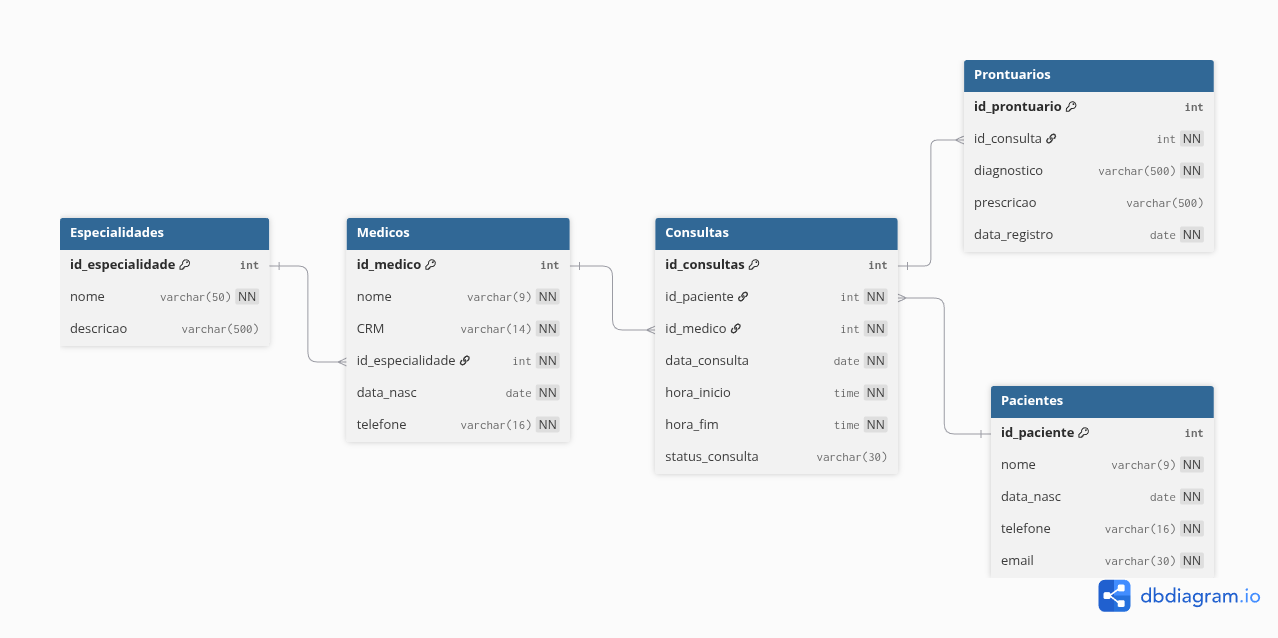
\includegraphics[width=1\linewidth]{db_conceitual.png}
    \caption{Esquema conceitual do banco \texttt{clinica\_db}. O marcador \textbf{NN} denota atributos com restrição de valor obrigatório (\textit{NOT NULL}).}
    \label{fig:conceitual}
\end{figure}

Ao longo deste documento, apresentaremos o processo de criação, manipulação e desenvolvimento de mecanismos que garantam o bom funcionamento do sistema.

\begin{alertbox}
\begin{center}
\textbf{Nota}    
\end{center}
Apresentaremos aqui apenas partes do código que merecem uma atenção especial, para visualizar o código completo, acesse o repositório no GitHub: https://github.com/L1nk404/Projeto-Aula-MySQL
\end{alertbox}

\newpage
\section{Desenvolvimento}
% DDL ==========================================================================
\subsection{Estrutura do Banco de Dados (DDL)}

Foram criadas cinco tabelas relacionadas entre si, conforme ilustrado na \textbf{Figura \ref{fig:conceitual} (p. \pageref{fig:conceitual})}.

Nesse subcapítulo daremos mais atenção à tabela \texttt{Consultas}, pois com ela podemos abordar elementos encontrados nas demais. Nela também adicionamos \texttt{CONSTRAINTS} por fins didáticos, pois, em ambos os casos de uso, seria mais efetivo\footnote{Numa situação de pequenos banco de dados com baixo volume de \texttt{INSERT} e \texttt{UPDATE}, pois \texttt{TRIGGERS} funcionam de forma procedural\cite{TRIGGER_PROC}.} aplicar apenas o uso de \texttt{TRIGGERS}. Veja o script abaixo:

\begin{lstlisting}[
    language=MySQL,
    caption={CREATE TABLE Consultas},
    label=lst:create-consultas-table
]
CREATE TABLE Consultas (
    id_consulta         INT PRIMARY KEY AUTO_INCREMENT,
    id_paciente         INT NOT NULL, 
    id_medico           INT NOT NULL,
    data_consulta       DATE NOT NULL, -- YYYY-MM-DD
    hora_inicio         TIME NOT NULL, -- hh:mm:ss
    hora_fim            TIME NOT NULL, -- hh:mm:ss
    status_consulta     VARCHAR(30), -- confirmado, cancelado, realizado, paci_ausente             

    CONSTRAINT chk_horario_valido CHECK 
        (hora_inicio >= '8:00:00' AND hora_inicio <= '17:00:00'),
    CONSTRAINT chk_horario_fim_valido CHECK 
        (hora_fim > hora_inicio AND hora_fim <= '18:00:00'),

    CONSTRAINT chk_status CHECK 
        (status_consulta IN ('confirmado', 'cancelado', 'realizado', 'paci_ausente')), -- apenas 4 valores são aceitos

    FOREIGN KEY(id_paciente) REFERENCES Pacientes(id_paciente) 
        ON UPDATE CASCADE 
        ON DELETE RESTRICT,
    FOREIGN KEY(id_medico) REFERENCES Medicos(id_medico) 
        ON UPDATE CASCADE 
        ON DELETE RESTRICT
);
\end{lstlisting}
\noindent

\subsubsection{Data Type} % DATA TYPE

A partir da linha 6 é possível perceber que 2 novos tipo de dados são usados, são eles:

\begin{enumerate}
    \item \texttt{DATE} - Uma data. O intervalo suportado é de \texttt{1000-01-01} até \texttt{9999-12-31}. O formato apresentado pelo MySQL para dados do tipo \texttt{DATE} é \texttt{YY-MM-DD} \cite{MySQL_DATE}.
    \item \texttt{TIME} - Um horário. O Intervalo suportado é de \texttt{-838:59:59.000000} até \texttt{838:59:59.000000}. O formato apresentado pelo MySQL para dados do tipo \texttt{TIME} é \texttt{hh:mm:ss} \cite{MySQL_DATE}.
\end{enumerate}

\subsubsection{CONSTRAINT} % CONTRAINT

Já da linha 10 até a linha 16 declaramos nossas \texttt{CONSTRAINT}. Aqui elas têm o papel de impedir que dados inválidos sejam inseridos.
\begin{itemize}
    \item \textbf{Linha 10 e 11} - Valida se o agendamento está sendo feito em horário de funcionamento da clínica.
    \item \textbf{Linha 12 e 13} - Valida se o horário estimado para o fim da consulta faz sentido, isto é, é depois do horário do início e deve ainda estar dentro do horário de funcionamento da clínica.
    \item \textbf{Linha 15 e 16} - Permite apenas 4 tipos de status para consultas, são eles:
        \begin{itemize}
            \item confirmado,
            \item cancelado,
            \item realizado,
            \item paci\_ausente 
        \end{itemize}
\end{itemize}


\subsubsection{Chave Estrangeiras} % CHAVE ESTRANGEIRA

Finalmente, das linhas 18 até a 23 referenciamos nossas chaves estrangeiras.

Assim, temos \texttt{id\_paciente} referenciado da tabela \texttt{Pacientes} e \texttt{id\_medico} referenciado da tabela \texttt{Medicos} respectivamente (\textbf{Figura \ref{fig:conceitual} p. \pageref{fig:conceitual}}). Temos duas opções adicionais para as chaves estrangeiras, são elas:
\begin{itemize}
    \item \textbf{CASCADE} - Seu papel é simples mas crucial. A opção \texttt{CASCADE} faz com que ações tomadas\footnote{Podem ser exclusão (\texttt{ON DELETE}) ou atualização (\texttt{ON UPDATE})} no registro da tabela pai sejam herdadas para todas as colunas filhas que possuem essa opção\cite{delete_cascade}. Aqui usamos \texttt{ON UPDATE}. Portanto, ao atualizar a chave pai, a chave herdada será também excluída.
    % 
    \item \textbf{RESTRICT} - Impede que ocorra a exclusão ou a atualização de um registro da tabela pai, caso ainda hajam registros na tabela filha. Uma exceção de violação de chave estrangeira é retornada. A verificação de integridade referencial é realizada antes de tentar executar a instrução \texttt{UPDATE} ou \texttt{DELETE}\cite{delete_cascade}.
    No script \ref{lst:create-consultas-table} usamos \texttt{ON DELETE}, logo, impedimos que o médico ou paciente seja excluído se ainda houver alguma consulta marcada.
\end{itemize}

\subsection{Alterações}

Podemos alterar colunas com o seguinte script:

\begin{lstlisting}[
    language=MySQL,
    caption=Alter Table,
    label=lst:alterTable
]
ALTER TABLE Prontuarios ADD validade DATE NOT NULL;
ALTER TABLE Prontuarios DROP COLUMN validade;  
\end{lstlisting}

Aqui na linha 1 adicionamos uma coluna do tipo \texttt{DATE} na tabela Prontuário, já na tabela 2 a excluímos. Podemos verificar através do comando \texttt{DESCRIBE}:

\begin{figure}[H]
    \centering
    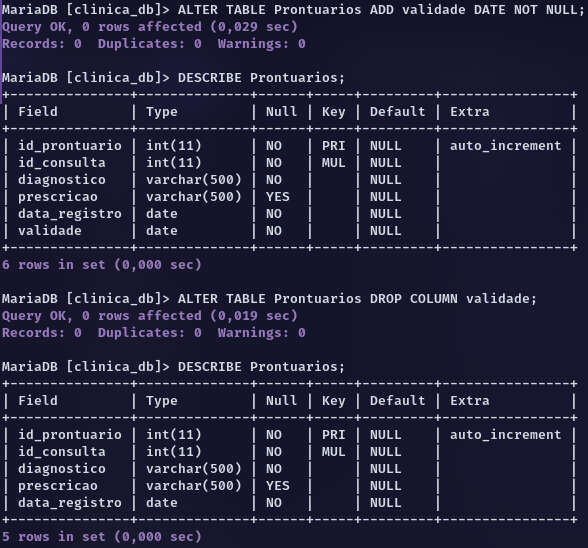
\includegraphics[width=0.85\linewidth]{Text/DDL/Describe.png}
    \caption{Alterações na tabela Prontuários}
    \label{fig:Describe}
\end{figure}

É possível também deletar tabelas no banco de dados com um simples \texttt{DROP TABLES}:

\begin{lstlisting}[
    language=MySQL,
    caption=Alter Table,
    label=lst:alterTable
]
CREATE TABLE teste (coluna_1 INT);
DROP TABLE teste;
\end{lstlisting}

O resultado pode ser visto a seguir:

\begin{figure}[H]
    \centering
    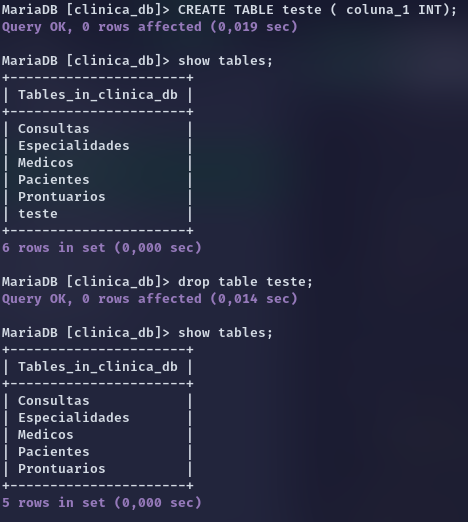
\includegraphics[width=0.50\linewidth]{Text/DDL/drop_table.png}
    \caption{Criação e Exclusão de tabela teste}
    \label{fig:drop_table}
\end{figure}

% DML ==========================================================================
\newpage
\section{Manipulação de Dados (DML)}
%
%
%
%
Esse capítulo tem uma proposta mais direta, aqui trataremos de alguns poucos comandos diretos para Manipulação de Dados, ou \textbf{DML}.

Para prosseguir, vamos primeiro popular nosso banco de dados com valores iniciais. Buscando simplicidade, nesta sessão focaremos nossos exemplos ao redor da tabela \texttt{Especialidades}. Todavia, é possível visualizar os dados inseridos nas demais na sessão de Apêndice (\textbf{Cap. \ref{subsec: DML} p. \pageref{subsec: DML}}). 

Usando o comando \texttt{INSERT} inserimos dados no campo \texttt{nome} e \texttt{descricao}:

\begin{lstlisting}[
    language=MySQL,
    caption=Perceba que não precisamos colocar valor para \texttt{id\_especialidade} por causa da opção \texttt{AUTO\_INCREMENT},
    label=insert_especialidade
]
INSERT INTO Especialidades 
    (nome, descricao) 
VALUES
    ('Cardiologia', 'Especialidade medica que trata doencas do coracao e sistema circulatorio'),
    ('Dermatologia', 'Especialidade medica que trata doencas da pele, cabelos e unhas'),
    ('Pediatria', 'Especialidade medica dedicada ao cuidado de criancas e adolescentes'),
    ('Ortopedia', 'Especialidade medica que trata doencas e deformidades do sistema musculoesqueletico'),
    ('Ginecologia', 'Especialidade medica que trata da saude do sistema reprodutor feminino'),
    ('Clinico Geral', 'Medico generalista que trata de problemas de saude diversos'),
    ('Campo para teste', 'Usaremos esse campo para testar os demais comandos');
\end{lstlisting}

Vamos agora mudar o nome do dado "Campo para Teste" para apenas "Teste". Antes disso, vamos verificar se ele foi inserido com sucesso, para isso, basta usarmos \texttt{SELECT * FROM Especialidades WHERE nome='Campo para teste';} :

\begin{figure}[H]
    \centering
    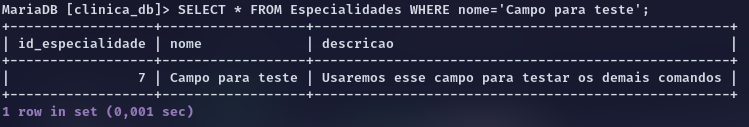
\includegraphics[width=1\linewidth]{Text//DML/campo_teste.png}
    \caption{\texttt{Campo para teste} antes das alterações}
    \label{fig:CampoTeste1}
\end{figure}

Agora, usando \texttt{UPDATE} alteraremos o nome:

\begin{lstlisting}[
    language=MySQL,
    caption=UPDATE nome,
    label=Update_especialidade
]
UPDATE Especialidades 
    SET nome = 'Teste'
WHERE
    nome = 'Campo para teste';;
\end{lstlisting}

Assim:

\begin{figure}[H]
    \centering
    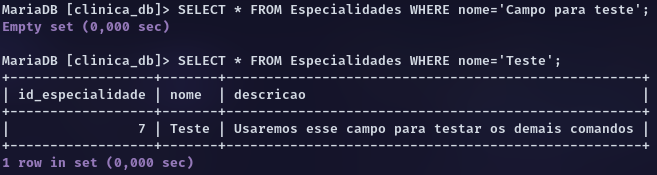
\includegraphics[width=1\linewidth]{Text//DML/campo_teste2.png}
    \caption{Perceba que não existe mais um dado com nome "Campo para Teste" pois o mesmo mudou para "Teste"}
    \label{fig:CampoTeste2}
\end{figure}

Finalmente vamos apagar o campo que mudamos, para isso basta usarmos \texttt{DELETE}:
\begin{lstlisting}[
    language=MySQL,
    caption=DELETE Teste,
    label=Update_especialidade
]
DELETE FROM Especialidades WHERE nome = 'Teste';
\end{lstlisting}

E então não temos mais esse registro em nossa tabela:

\begin{figure}[H]
    \centering
    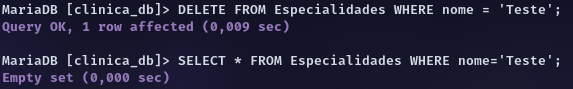
\includegraphics[width=1\linewidth]{Text/DML/Delete_teste.png}
    \caption{A ausência do valor no output indica que o dado não existe.}
\end{figure}


% Procedimentos e Funções ======================================================
\newpage
\section{Procedimentos e Funções}
%
%
\subsection{PROCEDURE}
\subsubsection{Planejamento}
Aqui criaremos um procedimento\footnote{Análogo a uma função do tipo \texttt{VOID} (pois procedimentos não retornam valores) numa linguagem de programação, um \texttt{PROCEDURE} ou procedimento é um bloco de código que pode ser armazenado e executado em um banco de dados\cite{Procedure}.} para agendar uma nova consulta, daremos a ele o nome de \texttt{Agendar}.

Para isso, serão necessários cinco parâmetros, são eles: \texttt{id\_paciente}, \texttt{id\_medico}, \texttt{data}, \texttt{hora\_inicio} e \texttt{hora\_fim}.

Dessa forma, o procedimento verificará se já existe alguma consulta marcada com o médico; em caso negativo, a consulta será agendada; em caso positivo, uma mensagem de erro aparecerá para o usuário. Abaixo é possível conferir o fluxograma do nosso procedimento:

\begin{figure}[H]
    \centering
    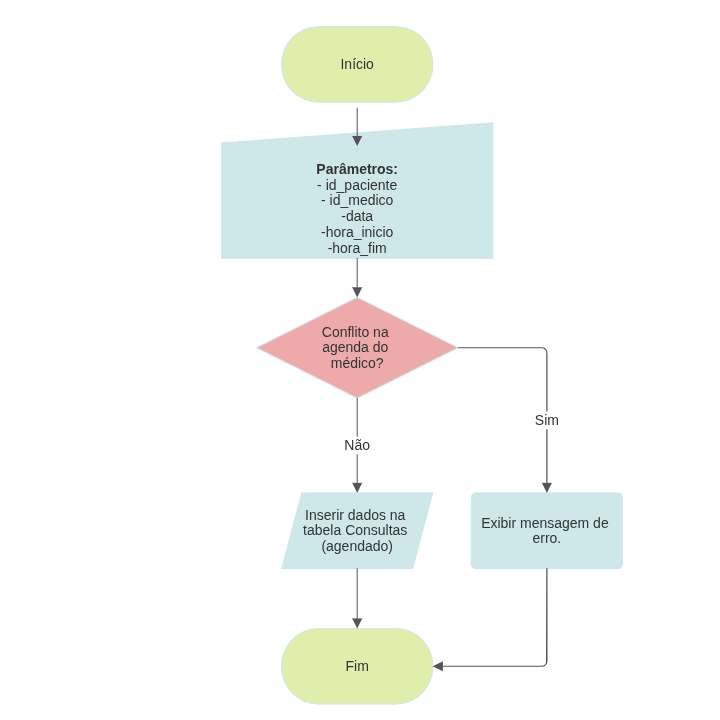
\includegraphics[width=0.75\linewidth]{Text/Proc/flowchart.png}
    \caption{Fluxograma da lógica do procedimento \texttt{Agendar}}
    \label{fig:agendar_flow}
\end{figure}

\newpage
\subsubsection{Execução}

Para declarar um procedimento, primeiro precisamos de um \texttt{DELIMITER}\footnote{Um delimitador (\texttt{DELIMITER}) pode ser entendido como uma notação que marca início e fim de um bloco de código, ele tem prioridade sobre o "\texttt{;}" , isto é, o código não termina com o "\texttt{;}"\ quando está dentro de um delimitador\cite{Delimiter}.}. Com isso começamos o código para nosso procedimento. Vamos dividi-lo em blocos mas é possível vê-lo por completo no Apêndice na subseção \textbf{\ref{subsec:proc} p. \pageref{subsec:proc}}.

\begin{lstlisting}[
    language=MySQL,
    caption=Declaração do procedimento e de variável
]
DELIMITER $$

CREATE PROCEDURE Agendar(
    IN p_id_paciente      INT,
    IN p_id_medico        INT,
    IN p_data_consulta    DATE,
    IN p_hora_inicio      TIME,
    IN p_hora_fim         TIME
)
BEGIN
DECLARE conflito_medico INT DEFAULT 0; 
\end{lstlisting}

Como estamos lidando com inserção de dados precisamos garantir a integridade dos mesmos, assim, usaremos \texttt{TRANSACTION}\footnote{Uma série de comandos \textbf{DML} com mecanismo de segurança de integridade que permitem cancelar toda a operação sem afetar os dados já escrito caso aconteça algum erro\cite{TRANSACTION}.}, logo, se acontecer algum erro durante a execução do procedimento, não há risco dos dados existente serem corrompidos.

\begin{lstlisting}[
    language=MySQl,
    caption=Verificação de conflitos no agendamento
]
-- Inicia a transacao
START TRANSACTION;

-- verifica data e hora sao validas
IF (p_data_consulta < CURDATE()
    OR
    p_data_consulta = CURDATE() AND p_hora_inicio < ADDTIME(CURTIME(), '01:00:00')
   ) THEN

    SIGNAL SQLSTATE '45000'
    SET MESSAGE_TEXT = 'Erro: Hora ou data nao validos!';
END IF;


-- Verifica conflito na agenda do medico
SELECT COUNT(*) INTO conflito_medico
FROM Consultas
WHERE id_medico = p_id_medico
    AND data_consulta = p_data_consulta
    AND status_consulta != 'cancelado' -- Ignora consultas canceladas
    AND ( 
        -- Conflito: nova consulta inicia durante uma existente
        (p_hora_inicio >= hora_inicio AND p_hora_inicio < hora_fim) 
        OR
        -- Conflito: nova consulta termina durante uma existente  
        (p_hora_fim > hora_inicio AND p_hora_fim <= hora_fim) 
        OR
        -- Conflito: nova consulta engloba uma existente
        (p_hora_inicio <= hora_inicio AND p_hora_fim >= hora_fim)
    );    
\end{lstlisting}

Acima temos duas verificações feitas para que o agendamento seja realizado.
\begin{itemize}
    \item \textbf{Linha 5 a 12} - Verifica se as datas são válidas usando funções nativas do MySQL como \texttt{CURDATE()} e \texttt{CURTIME()}, elas retornam a atual do servidor e o horário, respectivamente.
    \item \textbf{linha 16  a 30} - Verifica se o médico tem alguma consulta marcada para o dia e horário desejado. Note na linha 20 que caso a consulta esteja marcada como "\textbf{cancelado}", a verificação a ignora.
\end{itemize}

Finalmente temos:

\begin{lstlisting}[
    language=MySQL,
    caption=Final do código
    ]
-- Na ausencia de conflitos:
IF conflito_medico = 0 THEN
    INSERT INTO Consultas 
        (id_paciente, id_medico, data_consulta, hora_inicio, hora_fim, status_consulta)
    VALUES
        (p_id_paciente, p_id_medico, p_data_consulta, p_hora_inicio, p_hora_fim, 'agendado');

    COMMIT; -- Confirma a transicao
    
    SELECT 'Consulta agendada com sucesso!' AS Mensagem;
    SELECT * FROM Consultas WHERE 
        id_paciente=p_id_paciente AND 
        data_consulta = p_data_consulta AND 
        hora_inicio = p_hora_inicio;
    
ELSE -- Se conflito:
    ROLLBACK; -- Cancela as mudancas na transiction    
    
    SIGNAL SQLSTATE '45000'
    SET MESSAGE_TEXT = 'Erro: Medico ja possui uma consulta agendada nesse horario';
END IF;

END $$
DELIMITER ;
\end{lstlisting}

Aqui, inserimos ou não os dados na tabela. \begin{itemize}
    \item \textbf{Linha 2 a 14} - Caso não exista conflitos, a consulta é agendada com sucesso. Uma mensagem indicando que tudo foi bem sucedido aparece para o usuário juntamente com os dados da consulta agendada.
    \item \textbf{Linha 16 a 20} - Caso contrário, a consulta não é marcada. Uma mensagem de erro aparece para o usuário e a transação é cancelada. Aqui usamos o \texttt{SIGNAL\_STATE '45000'}, onde retornamos um código de erro, no caso, 45000 se refere a um caso genérico retornado pelo usuário\cite{MySQL_45000}.
\end{itemize}

\
\subsubsection{Testando o Procedimento}

Aqui testaremos o funcionamento do procedimento de forma simples. Primeiro vamos ver os dados que temos em Consulta:

\begin{figure}[H]
    \centering
    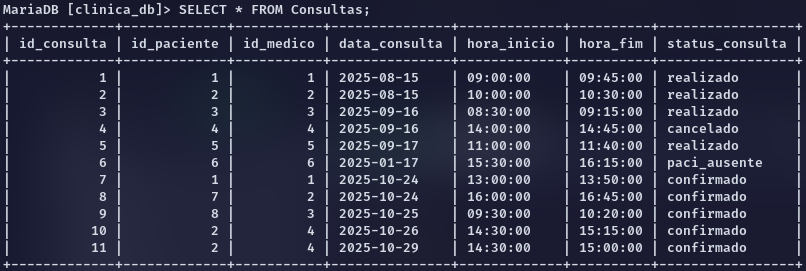
\includegraphics[width=0.8\linewidth]{Text//Proc/select_consulta.png}
    \caption{\texttt{SELECT * FROM Consultas;}}
    \label{fig:select_consulta}
\end{figure}

Agora vamos tentar inserir um dado de tal forma que aconteça um conflito na agenda, logo, usaremos o paciente 2 e o médico 4 para agendar uma consulta no dia 29/10/2025 as 14:50.
Depois vamos tentar inserir uma consulta com o mesmo paciente e médico no mesmo dia, porém as 16:00 horas.

\begin{figure}[H]
    \centering
    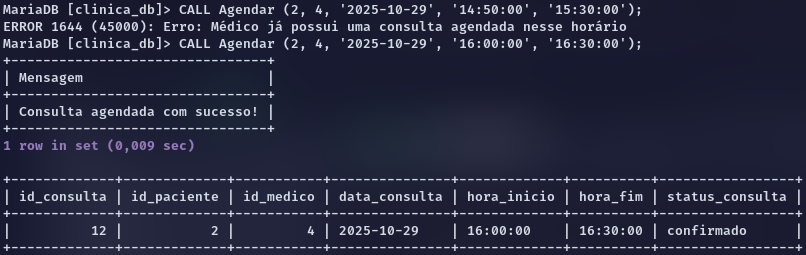
\includegraphics[width=1\linewidth]{Text//Proc/sucesso.png}
    \caption{Note que na primeira tentativa tivemos um erro e após escolher um horário disponível, tivemos sucesso.}
\end{figure}

\begin{alertbox}
    \begin{center}
        \textbf{Nota}
    \end{center}
    O teste aqui realizado não demonstra o completo funcionamento do procedimento, isto é, para todos os casos. Para isso, deveríamos fazer exaustivos testes englobando todas as possibilidades. Entretanto, o objetivo aqui é apenas demonstrativo.
\end{alertbox}

\subsection{Funções}
Nessa subseção trataremos de Funções. Aqui criaremos uma função simples, ela receberá um parâmetro que é o ano de nascimento de um paciente do tipo \texttt{DATE}, calculará com base na data do servidor sua idade, retornando assim, um valor inteiro.

Veja o código a seguir:

\begin{lstlisting}[
    language=MySQl,
    caption=Função Calc\_idade
]
DELIMITER $$

CREATE FUNCTION Calc_Idade (
    f_data_nascimento DATE
)

RETURNS INT
DETERMINISTIC

BEGIN 
    DECLARE idade INT;
    SET idade = TIMESTAMPDIFF(YEAR, f_data_nascimento, CURDATE());
    RETURN idade;
END; $$

DELIMITER ;
\end{lstlisting}

\begin{itemize}
    \item \textbf{Linha 3 a 8} - Aqui definimos a função, ela recebe um parâmetro \texttt{f\_data\_nascimento} do tipo \texttt{DATE}, e retornará um valor \texttt{INT}. Aqui também definimos a função como \texttt{DETERMINIST}\footnote{Uma função é dita determinista se, dadas as mesmas condições iniciais, isto é, os mesmos valores nos parâmetros, ela retornará o mesmo valor\cite{MySQL_deterministic}.}
    \item \textbf{Linha 11 a 13} - Aqui fazemos o cálculo da idade usando uma função nativa chamada \texttt{TIMESTAMPDIFF(Unidade, date\_time\_expr1, date\_time\_expr2)}, essa função retorna a diferença entre as datas inseridas. Veja a representação pictórica da função abaixo:

    \begin{figure}[H]
        \centering
        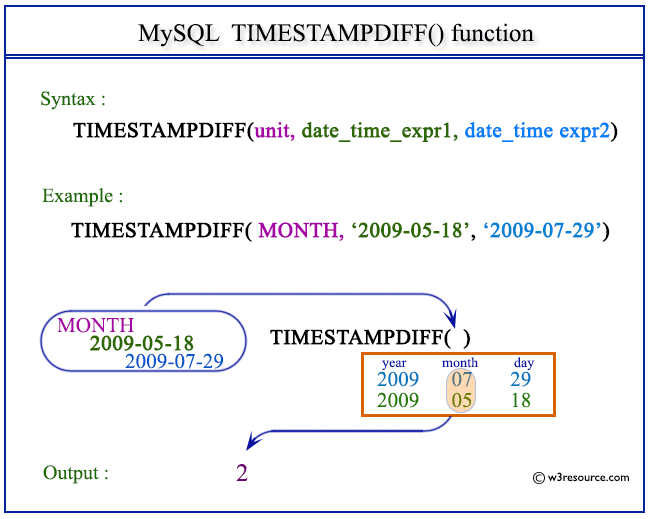
\includegraphics[width=0.75\linewidth]{Text//Proc/TIMESTAMPDIFF.png}
        \caption{Representação Pictórica de TIMESTAMPDIFF\cite{timestamp}}
        \label{fig:placeholder}
    \end{figure}
\end{itemize}

\subsubsection{Testando a Função com VIEW}
Vamos agora testar a função, primeiramente vamos analisar a idade de um paciente isolado, escolheremos o paciente de ID 3. Assim, com o comando \texttt{SELECT Calc\_Idade(data\_nasc) FROM Pacientes WHERE id\_paciente = 3;} temos:

\begin{figure}[H]
    \centering
    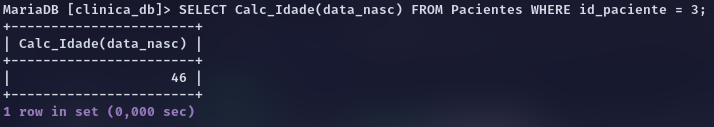
\includegraphics[width=1\linewidth]{Text//Proc/idade_3.png}
    \caption{\texttt{SELECT Calc\_Idade(data\_nasc) FROM Pacientes WHERE id\_paciente=3;}}
    \label{fig:placeholder}
\end{figure}

Agora, vamos usar a função para ver a idade de todos os pacientes. Como essa pode ser uma consulta usual, é interessante criarmos uma \texttt{VIEW}. Para isso usamos o comando a seguir:

\begin{lstlisting}[
    language=MySQL,
    caption=Criando \texttt{VIEW v\_paciente\_idade}
]
CREATE VIEW v_pacientes_idade AS
SELECT 
    id_paciente,
    nome,
    data_nasc,
    Calc_Idade(data_nasc) AS idade
FROM Pacientes;    
\end{lstlisting}

Assim, com um simples \texttt{SELECT * FROM v\_pacientes\_idade;}:

\begin{figure}[H]
    \centering
    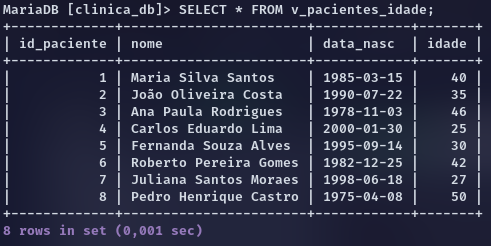
\includegraphics[width=0.75\linewidth]{Text//Proc/idade_table.png}
    \caption{\textbf{\texttt{SELECT * FROM v\_pacientes\_idade;}}}
\end{figure}

 Vamos aproveitar e criar um \texttt{VIEW} mais complexo onde podemos aplicar a função. Queremos agora um \textit{output} de todos os pacientes que tem consultas marcadas nos últimos 15 dias, e em vez de mostrarmos a data de nascimento, vamos pedir apenas a idade.

\begin{lstlisting}[
    language=MySQL,
    caption=Criando \texttt{VIEW v\_paciente\_agendados\_15}
]
CREATE VIEW v_pacientes_agendados_15 AS
SELECT 
    p.id_paciente,
    p.nome,
    Calc_Idade(data_nasc) AS 'Idade',
    c.data_consulta AS 'Data Consulta',
    c.status_consulta AS 'Status Consulta'
FROM Pacientes AS p
JOIN Consultas AS c
    ON p.id_paciente = c.id_paciente
WHERE
    TIMESTAMPDIFF(DAY, c.data_consulta, CURDATE()) <= 15;
\end{lstlisting}

Assim:

\begin{figure}[H]
    \centering
    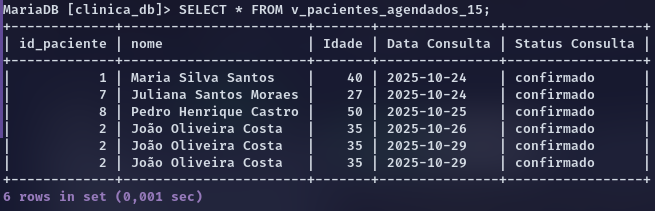
\includegraphics[width=1\linewidth]{Text//Proc/image.png}
    \caption{\texttt{VIEW v\_pacientes\_agendados\_15}}
\end{figure}







\newpage
\newpage
\section{Apêndice}\label{sec:Apendice}
\subsection{Manipulação de Dados (DML)}\label{subsec: DML}

\begin{figure}[H]
    \centering
    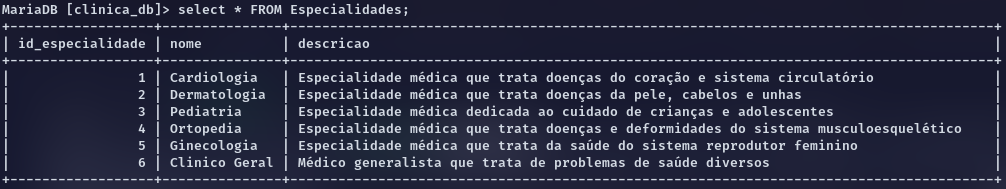
\includegraphics[width=1\linewidth]{Text/DML/Especialidades.png}
    \caption{Tabela Especialidades - \texttt{SELECT * FROM Especialidades;}}
    \label{fig:Especialidades}
\end{figure}

\begin{figure}[H]
    \centering
    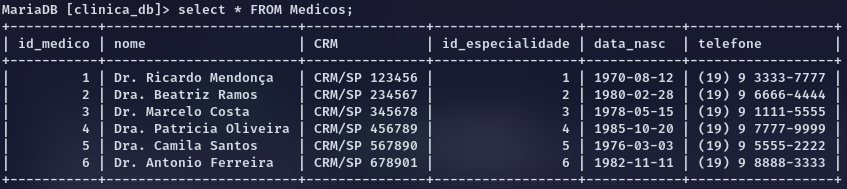
\includegraphics[width=1\linewidth]{Text/DML/Medicos.png}
    \caption{Tabela Medicos - \texttt{SELECT * FROM Medicos;}}
    \label{fig:Medicos}
\end{figure}

\begin{figure}[H]
    \centering
    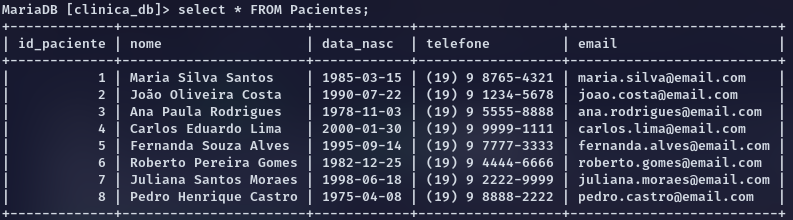
\includegraphics[width=1\linewidth]{Text/DML/Pacientes.png}
    \caption{Tabela Pacientes - \texttt{SELECT * FROM Pacientes;}}
    \label{fig:Pacientes}
\end{figure}

\begin{figure}[H]
    \centering
    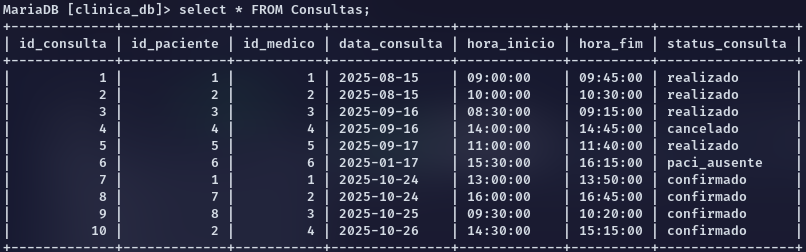
\includegraphics[width=1\linewidth]{Text/DML/Consultas.png}
    \caption{Tabela Consultas - \texttt{SELECT * FROM Consultas;}}
    \label{fig:Especialdiades}
\end{figure}

\begin{figure}[H]
    \centering
    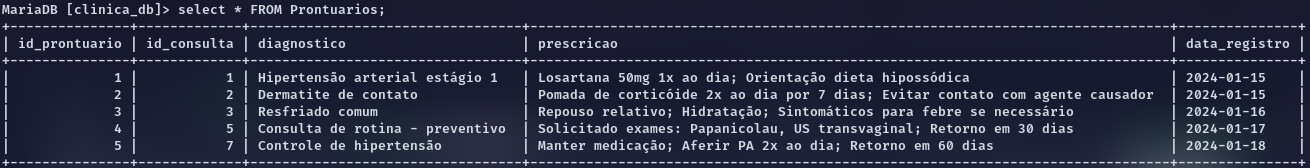
\includegraphics[width=1\linewidth]{Text/DML/Prontuarios.png}
    \caption{Tabela Prontuarios - \texttt{SELECT * FROM Prontuarios;}}
    \label{fig:Prontuarios}
\end{figure}

\newpage
\subsection{Procedimentos e Funções}\label{subsec:proc}
\begin{lstlisting}[
    language=MySQL,
    caption=Script para criação do procedimento \texttt{Agendar},
    label=AgendarProc
]
DELIMITER $$

CREATE PROCEDURE Agendar(
    IN p_id_paciente      INT,
    IN p_id_medico        INT,
    IN p_data_consulta    DATE,
    IN p_hora_inicio      TIME,
    IN p_hora_fim         TIME
)
BEGIN
DECLARE conflito_medico INT DEFAULT 0; 

-- Inicia a transacao
START TRANSACTION;

-- verifica data e hora sao validas
IF (p_data_consulta < CURDATE()
    OR
    p_data_consulta = CURDATE() AND p_hora_inicio < ADDTIME(CURTIME(), '01:00:00')
   ) THEN

    SIGNAL SQLSTATE '45000'
    SET MESSAGE_TEXT = 'Erro: Hora ou data nao validos!';
END IF;

-- Verifica conflito na agenda do medico
SELECT COUNT(*) INTO conflito_medico
FROM Consultas
WHERE id_medico = p_id_medico
    AND data_consulta = p_data_consulta
    AND status_consulta != 'cancelado' -- Ignora consultas canceladas
    AND ( 
        -- Conflito: nova consulta inicia durante uma existente
        (p_hora_inicio >= hora_inicio AND p_hora_inicio < hora_fim) 
        OR
        -- Conflito: nova consulta termina durante uma existente  
        (p_hora_fim > hora_inicio AND p_hora_fim <= hora_fim) 
        OR
        -- Conflito: nova consulta engloba uma existente
        (p_hora_inicio <= hora_inicio AND p_hora_fim >= hora_fim)
    );    

-- Na ausencia de conflitos:
IF conflito_medico = 0 THEN
    INSERT INTO Consultas 
        (id_paciente, id_medico, data_consulta, hora_inicio, hora_fim, status_consulta)
    VALUES
        (p_id_paciente, p_id_medico, p_data_consulta, p_hora_inicio, p_hora_fim, 'confirmado');

    COMMIT; -- Confirma a transicao
    
    SELECT 'Consulta agendada com sucesso!' AS Mensagem;
    SELECT * FROM Consultas WHERE 
        id_paciente=p_id_paciente AND 
        data_consulta = p_data_consulta AND 
        hora_inicio = p_hora_inicio;
    
ELSE -- Se conflito:
    ROLLBACK; -- Cancela as mudancas na transiction    
    
    SIGNAL SQLSTATE '45000'
    SET MESSAGE_TEXT = 'Erro: Medico ja possui uma consulta agendada nesse horario';
END IF;

END $$
DELIMITER ;
\end{lstlisting}

\newpage
\begin{thebibliography}{99}
\addcontentsline{toc}{section}{Referências}
    \bibitem{trybe} MARTINS, F. \textbf{SGBD: o que é, como funciona a arquitetura e 5 exemplos}!  Trybe, 2022.
    \bibitem{TRIGGER_PROC} \textbf{Triggers em Banco de Dados: Entenda em Detalhes}. Skills Tecnologias, 2024.
    \bibitem{MySQL_DATE} ORACLE. \textbf{MySQL Documentation} - 13.2.1 Date and Time Data Type Syntax. MySQL, 2025.
    \bibitem{delete_cascade} REIS, F. \textbf{ON DELETE CASCADE e Opções de Chave Estrangeira no MySQL}. Bóson Treinamentos em Ciência da Tecnologia, 2018.
    \bibitem{Procedure} MONUTI, D. \textbf{O que é uma Procedure em SQL? E como criar Procedure no SQL} Hashtag Treinamentos. 
    \bibitem{Delimiter} GAIKWAD, T. \textbf{MySQL Delimiter – A Complete Guide}. MySQL Code, 2022
    \bibitem{TRANSACTION} GeeksforGeeks \textbf{MySQL Transaction}. Geeks for Geeks, 2025
    \bibitem{MySQL_45000} ORACLE. \textbf{MySQL Documentation} - 15.6.7.5 SIGNAL Statement. MySQL, 2025.
    \bibitem{MySQL_deterministic} ORACLE. \textbf{MySQL Documentation} - 10.2.1.20 Function Call Optimization. MySQL, 2025.
    \bibitem{timestamp} W3RESOURCE - \textbf{MySQL TIMESTAMPDIFF() function}. w3resource, 2024.    
    % \bibitem{w3schools} \textbf{MySQL Tutorial}. w3schools.com
    % \bibitem{MySQL_dod} \textbf{MySQL Documentation}. MySQL.com/doc
    % \bibitem{ref2} \textbf{TAXA METABÓLICA BASAL: O QUE É E COMO PODE SER CALCULADA}. Essential Nutrition, 2022
    % \bibitem{ref3}
    % BELCIT, Ivan. \textbf{O que é Cross-Site Scripting (XSS)?}. avast.com, 2020.
\end{thebibliography}
\end{document}

https://app.diagrams.net app de fluxogramas